\section{WDIAS Database Structure}
\label{se:db_struct}

The foundation of the \acrshort{wdias} is data-centric. We need to look into the weather data timeseries deeply to understand the underline design decisions of the \acrshort{wdias} database structure.

\paragraph{Timeseries}-- \emph{A timeseries is simply a series of data points ordered in time}. In the weather domain, we are interested in observation and forecasting timeseries data. Each timeseries, the data points can be formed in different formats as well. For example, scalar (0D), vector (1D), grid (2D), and polygon (2D).

Based on the above interpretation, a timeseries have data points ordered in time. Other than that, timeseries have additional information that is known as \emph{timeseries metadata}, which can use to identify one timeseries from another uniquely. As an example, we can place a weather station on a \emph{location}, and it can measure different types of weather data that are called \emph{parameters} such as temperature, precipitation, and wind direction. Each parameter can produce different timeseries. Even we can use the location as metadata to identify the timeseries, but that is not enough to distinctly identify the parameters. Thus, we need to use a set of attributes to identify a timeseries uniquely. In the next \cref{subse:timeseries_key_attributes}, we describe key attributes that are used by the \acrshort{wdias} to identify a timeseries uniquely.


%%%%%%%%%%%%%%%%%%%%%%%%%%%%%%%%%%%%%%%%%%%%%%%%%%%%%%%%%%%%%%%%%%%%%%%%%%%%%%%%
\subsection{Key Attributes of Timeseries}
\label{subse:timeseries_key_attributes}
\paragraph{Module ID}-- String field which describe the source of the data generated. e.g., hec-hms, flow2d, weather-station, etc

\paragraph{Value Type}-- Scalar, Vector, Grid are the Value Types that are interested in the \acrshort{wdias}.

\paragraph{Location}-- Location of the timeseries. All locations have a unique String identifier called \emph{locationId}. Further, two types of location types are interested in the \acrshort{wdias}, namely:
\begin{itemize}
  \item \emph{Point locations}-- Contains a name that is human readable. lat and lon of the location on the earth surface.
\begin{lstlisting}[language=Python]
{
    "locationId": "wdias-hanwella",
    "name": "Hanwella",
    "lat": 6.909722222,
    "lon": 80.08166667
}
\end{lstlisting}
  \item \emph{Regular Grid locations} -- Contains a name that is human readable. The grid presents by dividing into equal size cells. Thus, it needs the number of rows and columns. 
  And the location of the first cell and the width and height of it.
\begin{lstlisting}[language=Python]
{
    "locationId": "wdias_kelani_basin",
    "description": "Kelani Basin",
    "rows": 120,
    "columns": 139,
    "geoDatum": "Kandawala",
    "gridFirstCell": {
        "firstCellCenter": {
            "x": 397074.0,
            "y": 504875.0
        },
        "xCellSize": 250.0,
        "yCellSize": 250.0
    }
}
\end{lstlisting}
  \item \emph{Irregular Grid locations} -- (endpoints are available within the WDIAS system, but skipped since it is out of the interest of the scope.)
\end{itemize}

\paragraph{Parameter}
Parameter describes the variable measuring against a location. All parameters should have a unique string identifier called \emph{parameterId}. A parameter can be used in multiple locations. While defining a parameter, three required fields need to be provided, such as variable, unit, and \emph{parameterType}.

\begin{itemize}  
  \item \emph{Variable} -- Nature of the variable measuring. Example Precipitation, Temperature and Water Level etc
  \item \emph{Unit} -- metric unit of measuring
  \item \emph{Parameter Type} -- Should be one of Instantaneous, Accumulative, or Mean
\begin{lstlisting}[language=Python]
{
  "parameterId": "O.Precipitation",
  "variable": "Precipitation",
  "unit": "mm",
  "parameterType": "Instantaneous"
}
\end{lstlisting}
\end{itemize}

\subsubsection{Timeseries Type}
Users can define timeseries type while setup the system. We determined the following types as the default values. Timeseries type can be a combination of a source followed by category:
\begin{itemize}
  \item Sources - External or simulated. \emph{External} means whether timeseries is taken from an external source, and \emph{simulated} means it generated by simulations of the users.
  \item Category - Historical or forecast. \emph{Historical} means whether timeseries have continuous data such as observations from a weather station. \emph{forecast} means discrete set of timeseries data produce by forecasting.
\end{itemize}

\paragraph{Time Step}-- All TimeSteps has a unique String identifier called timeStepId. The unit should be one of Second, Minute, Hour, Day, Week, Month, Year, or NonEqualDistance. One of multipliers or dividers can be used to define the interval between each measurement.
\begin{lstlisting}[language=Python]
{
    "timeStepId": "each_min",
    "unit": "Minute",
    "multiplier": 1,
    "divider": 0
}
\end{lstlisting}

Among the above key attributes; Location, Parameter and Time Step attributes are composite attributes. But each of them has a unique identifier.
Given that, a timeseries can uniquely identify by \emph{moduleId, valueType, parameterId, locationId, timeseriesType and timeStepId}.
\begin{lstlisting}[language=Python]
{
	"moduleId": "HEC-HMS",
	"valueType": "Scalar",
	"parameterId": "O.Precipitation",
	"locationId": "wdias_hanwella",
	"timeseriesType": "External_Historical",
	"timeStepId": "each_hour",
}
\end{lstlisting}

%%%%%%%%%%%%%%%%%%%%%%%%%%%%%%%%%%%%%%%%%%%%%%%%%%%%%%%%%%%%%%%%%%%%%%%%%%%%%%%%
Even if a timeseries consists of data points in time ordered, the data for each data point can vary based on the valueType. The scalar data point consists of a single value. And the vector data point consists of two values, such as magnitude and the direction of the vector. But for Grid data, a point can consist of multiple values. To store data efficiently, we used a set of different databases based on the advantage of using them for each valueType. Other attributes do not have much impact on classifying the timeseries data.

It is difficult to search for the timeseries data if those are stored over multiple data sources and trying to avoid having duplicates. ,it adds low overhead to have a single data source to look into while searching for the timeseries metadata. The efficiency of searching for timeseries metadata can increase by using a caching mechanism. To support search queries with lower latency, we used an index for the fast search for timeseries metadata, and a geo-based index to support geo-based search queries.

Many modern database systems give a higher performance on a specific type of application. Thus, we need to use the correct database system based on application requirements. Considering the aforementioned database requirements, we cannot get all of the benefits using a single general database system available. Thus, we created a database structure after carefully choosing database systems per the system requirements and combining their capabilities. According to the design principle of microservices architecture, we created microservice for each of the valueType. Here we followed the concept of \emph{database per service} as described in in \cref{subse:database_per_service}. In \cref{sebse:wdias_microservices}, those microservices are grouped as \emph{adapters} that share an \acrshort{api} to interact with while keeping the persistent data private.

\begin{figure}[htp]
    \centering
    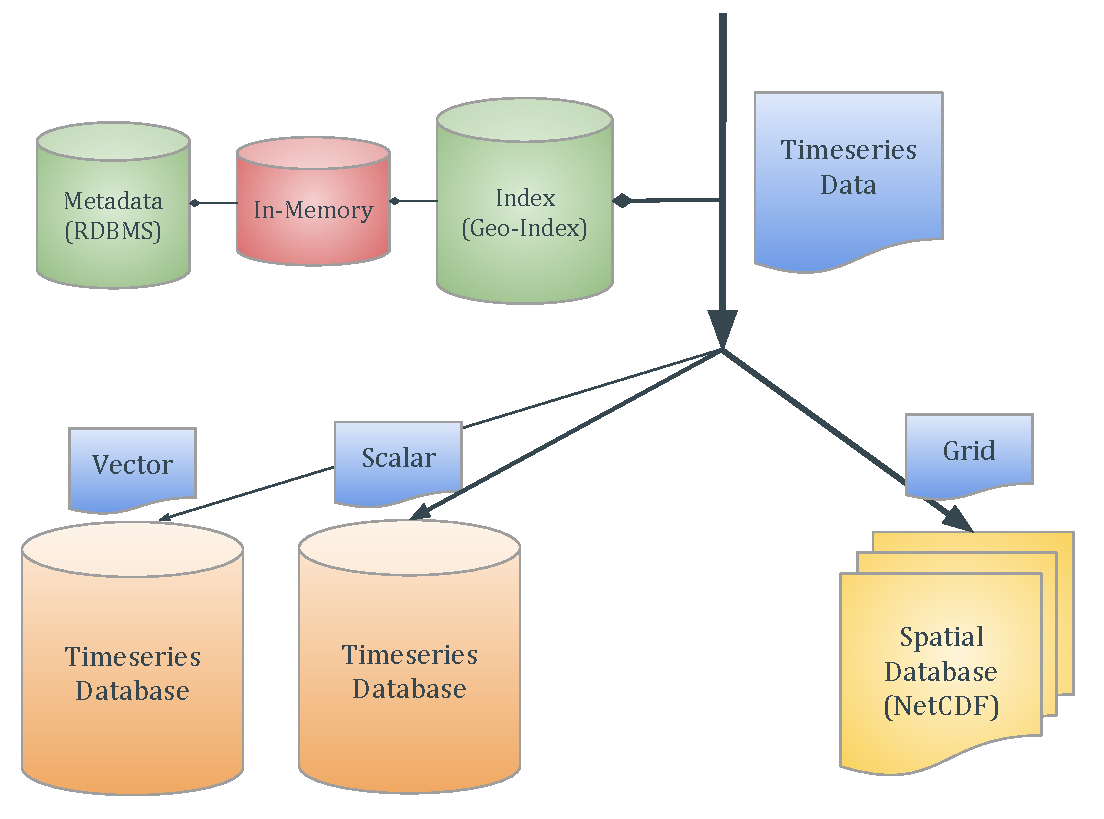
\includegraphics[width=0.8\textwidth]{method/microservice/wdias_database_structure.pdf}
    \caption{\acrshort{wdias} database structure}
    \label{fi:database_structure}
\end{figure}

\cref{fi:database_structure} shows the \acrshort{wdias} database structure.
The following sections describe the database structure of \acrshort{wdias} with compare to the design with more details on how is support the microservice architecture.

%%%%%%%%%%%%%%%%%%%%%%%%%%%%%%%%%%%%%%%%%%%%%%%%%%%%%%%%%%%%%%%%%%%%%%%%%%%%%%%%
\subsection{Timeseries Metadata Storage}
\label{subse:mysql}

To reduce the overhead while searching for timeseries and handling duplicates, we used a timeseries metadata store. Since metadata consists of multiple key attributes, the data can be efficiently stored using a \acrfull{rdbms}. It helps to store data without any duplicates and optimize the data with normalization. As an example, the parameter attribute can only have a dozen possible values. Using an \acrshort{rdbms}, those values can be stored once and reuse with defining timeseries against location via references.

We used SQL as the \acrshort{rdbms}. Since one of \acrshort{wdias} main goals is to use open source tools, it used MySQL as a persistent database for storing timeseries metadata described above. One MySQL instance used only for adapter-metadata service. Other than that, another MySQL instance used for adapter-extension. We will explain in more detail in \cref{se:data_preprocess}. We used MySQL only for the above services, and those database instances keep the consistency of the schema for timeseries metadata and extension metadata. Further, we used an In-Memory database instance for caching the requested metadata to reduce the load on the MySQL database instances while repeated queries. Other than MySQL, many open-source SQL databases can be used to replace the same functionality.

%%%%%%%%%%%%%%%%%%%%%%%%%%%%%%%%%%%%%%%%%%%%%%%%%%%%%%%%%%%%%%%%%%%%%%%%%%%%%%%%
\subsection{In-Memory Database}
\label{subse:redis}

We used Redis \cite{redisRedisDocumentation} as the In-Memory database since it is a widely used database system with excellent support. It also supports Publisher Subscriber capabilities as an inbuilt feature. Redis is an open-source (BSD licensed). Clustering is available for scalability. Redis uses in-memory caching for fast access to the frequent access data in adapter-metadata and adapter-extension. Other than that, adapter-status uses Redis as a key-value pair store to maintain the status for async requests handling while storing grid data. The adapter-extension uses Redis's Publisher Subscriber capabilities to create a cronjob in extension-scheduler when a new extension creates with a trigger on time during data preprocessing.

%%%%%%%%%%%%%%%%%%%%%%%%%%%%%%%%%%%%%%%%%%%%%%%%%%%%%%%%%%%%%%%%%%%%%%%%%%%%%%%%
\subsection{Timeseries Database}
\label{subse:influxdb}

Among several timeseries open source databases, InfluxDB \cite{influxdbInfluxDBDocumentation} uses a unique database indexing algorithm to gain higher performance while storing timeseries data when compared to other modern databases available. Also, it has better support, higher usage, and following supports;

\begin{itemize}
  \item Open timeseries DB with MIT license
  \item Support SQL-Like query language
  \item Clustering available with a commercial version
\end{itemize}

Other than InfluxDB, the ElasticSearch database can be used, but it mainly uses indexing for searching. InfluxDB allows us to change the read/write behavior and indexing mechanism via database configurations. Further, users can use the commercial version of InfluxDB to gain more performance, like database sharding and replicas.

Two individual instances of InfluxDB used for adapter-scalar and adapter-vector services in the \acrshort{wdias} system. For the scalability, the system uses \emph{database per service}, as mentioned in \cref{subse:database_per_service}. If users want further performance, the database can split into another set of partitions based on other key attributes based on the Z-axis scaling described in \cref{subse:scale_cube}. As an example, scalar and vector adapters can further split into more services based on other key attributes such as timeseriesType.

%%%%%%%%%%%%%%%%%%%%%%%%%%%%%%%%%%%%%%%%%%%%%%%%%%%%%%%%%%%%%%%%%%%%%%%%%%%%%%%%
\subsection{Network Common Data Form}
\label{subse:netcdf}

\acrshort{netCDF} \cite{unidataUnidataNetCDF} is a self-describing, machine-independent data format that supports the creation, access, and sharing of array-oriented scientific data. Moreover, NetCDF also supports parallel file access. NetCDF is widely used in the scientific domain due to the capability of storing multi-dimensions data efficiently and flexibly. Thus, we used NetCDF for storing the grid data due to its capability of storing array-oriented scientific data efficiently when compared to other database systems.

%%%%%%%%%%%%%%%%%%%%%%%%%%%%%%%%%%%%%%%%%%%%%%%%%%%%%%%%%%%%%%%%%%%%%%%%%%%%%%%%
\subsection{Document-oriented Database}
\label{subse:mongodb}

To provide fast geo-search queries, we have to use a database system that supports geo indexing. We used MongoDB, which is a document-oriented database with Geo indexing capabilities. Also, MongoDB \cite{mongodbMongoDBManual} is a general-purpose, document-based, distributed database, and supports: 

\begin{itemize}
  \item Supports query operations on geospatial data \cite{mongodbMongoDBManual}
  \item Clustering and Sharding available for scalability and reliability
\end{itemize}

We used MongoDB geospatial features to support Geo queries in the \acrshort{wdias}. Also, we indexed the timeseries metadata with other indexing features to serve external timeseries metadata queries. If particular timeseries metadata not present in the adapter-query, then fetch metadata from the adapter-metadata and indexed in the MongoDB. Vise a versa; when a new timeseries created in the adapter-metadata, it triggers an event to index metadata in the adapter-query.
Here we used the \emph{Y-axis scaling} concept by splitting metadata search into multiple services. Within the system, it uses In-Memory database cache to support internal metadata access, and external search queries fulfill by the adapter-query with using MongoDB.
